\section{Transformada de Radon y retroproyección}
\label{RadonBackprojection}

Sea $f\in\mathcal S(\mathbb R^2)$. Para $t\in\mathbb R$ y $\theta\in[0,\pi)$, la transformada de Radon de $f$ se define por
\[
(\mathcal Rf)(t,\theta)
=
\int_{\mathbb R}
f\bigl(t\omega(\theta)+s\omega^\perp(\theta)\bigr)\,ds.
\]
Esta definición coincide con la integral de $f$ sobre la recta $L(t,\theta)$. La transformada de Radon sobre funciones de Schwartz se presenta en Helgason \cite{helgason1999} y Natterer \cite[Sec.~II.1, pp.~9--10]{natterer2001}. Allí pueden aparecer convenciones de parametrización y normalización distintas.\\

Al variar $t$ y $\theta$, los valores $(\mathcal Rf)(t,\theta)$ se organizan en el plano de datos. Para un punto $x_0$, su traza en el sinograma satisface $t(\theta)=x_0\cdot\omega(\theta)$. La Figura~\ref{fig:sinograma-diagrama} ilustra cómo una estructura puntual del objeto genera una curva en el sinograma.

\begin{figure}[htbp]
\centering
\resizebox{0.88\textwidth}{!}{\shorthandoff{<>}
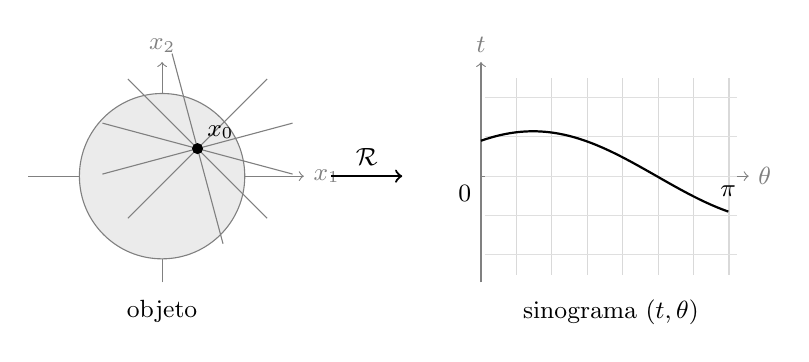
\begin{tikzpicture}[font=\small]
    \begin{scope}
        \draw[->, thin, gray] (-1.7,0) -- (1.8,0) node[right] {$x_1$};
        \draw[->, thin, gray] (0,-1.35) -- (0,1.45) node[above] {$x_2$};
        \draw[fill=black!8, draw=black!50] (0,0) circle (1.05);
        \coordinate (Xzero) at (0.45,0.35);
        \foreach \a in {15,45,75,105,135} {
            \draw[thin, gray] (Xzero) ++(\a+90:1.25) -- ++(\a-90:2.5);
        }
        \fill (Xzero) circle (2pt) node[above right] {$x_0$};
        \node[below] at (0,-1.45) {objeto};
    \end{scope}

    \draw[->, thick] (2.15,0) -- (3.05,0) node[midway, above] {$\mathcal R$};

    \begin{scope}[xshift=4.05cm]
        \draw[->, thin, gray] (0,0) -- (3.4,0) node[right] {$\theta$};
        \draw[->, thin, gray] (0,-1.35) -- (0,1.45) node[above] {$t$};
        \foreach \x in {0.45,0.9,...,3.15} {
            \draw[thin, gray!30] (\x,-1.25) -- (\x,1.25);
        }
        \foreach \y in {-1.0,-0.5,0,0.5,1.0} {
            \draw[thin, gray!25] (0.05,\y) -- (3.25,\y);
        }
        \draw[thick, black, domain=0:3.1416, samples=80, variable=\u]
            plot ({\u}, {0.45*cos(\u r)+0.35*sin(\u r)});
        \node[below left] at (0,0) {$0$};
        \node[below] at (3.14,0) {$\pi$};
        \node[align=center, below] at (1.65,-1.45) {sinograma $(t,\theta)$};
    \end{scope}
\end{tikzpicture}
\shorthandon{<>}
}
\caption{Formación esquemática del sinograma a partir de proyecciones paralelas. Elaboración propia.}
\label{fig:sinograma-diagrama}
\end{figure}

La linealidad se sigue directamente de la linealidad de la integral: para $f_1,f_2\in\mathcal S(\mathbb R^2)$ y escalares $a,b$,
\[
\mathcal R(af_1+bf_2)=a\mathcal Rf_1+b\mathcal Rf_2.
\]

Para identificar la retroproyección como adjunto formal, sea $D=\mathbb R\times(0,\pi)$. Para $u,v\in L^2(D)$ definimos el producto interno del espacio de datos por
\[
\langle u,v\rangle_{\mathrm{datos}}
=
\int_0^\pi\int_{\mathbb R}
u(t,\theta)\overline{v(t,\theta)}\,dt\,d\theta.
\]
Para $p\in L^1(\mathbb R^2)$ y $q\in L^\infty(\mathbb R^2)$ usamos la pareja de dualidad del espacio de imagen
\[
\langle p,q\rangle_{\mathrm{imagen}}
=
\int_{\mathbb R^2}p(x)\overline{q(x)}\,dx.
\]

Tomamos ahora $g\in C_c^\infty(D)$. Entonces $\mathcal Rf,g\in L^2(D)$ y $f\in L^1(\mathbb R^2)$. Definimos la retroproyección de $g$ por
\[
(\mathcal R^*g)(x)
=
\int_0^\pi
g(x\cdot\omega(\theta),\theta)\,d\theta.
\]
Además, $\mathcal R^*g\in L^\infty(\mathbb R^2)$, pues
\[
\|\mathcal R^*g\|_{L^\infty}
\leq
\pi\|g\|_{L^\infty}.
\]
Por consiguiente, en las parejas anteriores se toman concretamente $u=\mathcal Rf$, $v=g$, $p=f$ y $q=\mathcal R^*g$. Usando el cambio de variables
\[
x=t\omega(\theta)+s\omega^\perp(\theta),
\qquad dx=dt\,ds,
\]
para cada $\theta$, se obtiene
\[
\begin{aligned}
\langle\mathcal Rf,g\rangle_{\mathrm{datos}}
&=
\int_0^\pi\int_{\mathbb R}
(\mathcal Rf)(t,\theta)
\overline{g(t,\theta)}\,dt\,d\theta \\
&=
\int_{\mathbb R^2}
f(x)
\overline{
\left(
\int_0^\pi
g(x\cdot\omega(\theta),\theta)\,d\theta
\right)}\,dx \\
&=
\langle f,\mathcal R^*g\rangle_{\mathrm{imagen}}.
\end{aligned}
\]
Por tanto, la retroproyección $\mathcal R^*$ definida arriba es el adjunto formal de $\mathcal R$ con respecto a las medidas $dt\,d\theta$ y $dx$. La misma fórmula se empleará siempre que la integral angular esté bien definida. No se está afirmando aquí que ya se haya construido un operador acotado entre espacios $L^2$ completos. Para resultados de dualidad y retroproyección en un marco funcional más amplio puede consultarse Natterer \cite[Sec.~II.1, Thm.~1.3, pp.~13--15]{natterer2001}. Kuchment también desarrolla la retroproyección, aunque usa la notación $\mathcal R^\#$ y convenciones con integración angular diferentes \cite[Sec.~5.6, pp.~34--36]{kuchment2014}.
